% This is "sig-alternate.tex" V2.1 April 2013
% This file should be compiled with V2.5 of "sig-alternate.cls" May 2012
%
% This example file demonstrates the use of the 'sig-alternate.cls'
% V2.5 LaTeX2e document class file. It is for those submitting
% articles to ACM Conference Proceedings WHO DO NOT WISH TO
% STRICTLY ADHERE TO THE SIGS (PUBS-BOARD-ENDORSED) STYLE.
% The 'sig-alternate.cls' file will produce a similar-looking,
% albeit, 'tighter' paper resulting in, invariably, fewer pages.
%
% ----------------------------------------------------------------------------------------------------------------
% This .tex file (and associated .cls V2.5) produces:
%       1) The Permission Statement
%       2) The Conference (location) Info information
%       3) The Copyright Line with ACM data
%       4) NO page numbers
%
% as against the acm_proc_article-sp.cls file which
% DOES NOT produce 1) thru' 3) above.
%
% Using 'sig-alternate.cls' you have control, however, from within
% the source .tex file, over both the CopyrightYear
% (defaulted to 200X) and the ACM Copyright Data
% (defaulted to X-XXXXX-XX-X/XX/XX).
% e.g.
% \CopyrightYear{2007} will cause 2007 to appear in the copyright line.
% \crdata{0-12345-67-8/90/12} will cause 0-12345-67-8/90/12 to appear in the copyright line.
%
% ---------------------------------------------------------------------------------------------------------------
% This .tex source is an example which *does* use
% the .bib file (from which the .bbl file % is produced).
% REMEMBER HOWEVER: After having produced the .bbl file,
% and prior to final submission, you *NEED* to 'insert'
% your .bbl file into your source .tex file so as to provide
% ONE 'self-contained' source file.
%
% ================= IF YOU HAVE QUESTIONS =======================
% Questions regarding the SIGS styles, SIGS policies and
% procedures, Conferences etc. should be sent to
% Adrienne Griscti (griscti@acm.org)
%
% Technical questions _only_ to
% Gerald Murray (murray@hq.acm.org)
% ===============================================================
%
% For tracking purposes - this is V2.0 - May 2012

%\documentclass[EPiC,debug]{easychair}
\documentclass[EPiCempty]{easychair}
\pagestyle{plain}

\usepackage{hyperref}
\usepackage{graphicx}
\usepackage{multirow}
\usepackage{mathptmx}
\usepackage{listings}
\usepackage{latexsym}
\usepackage{amsthm}
\usepackage{empheq}
\usepackage{geometry}
\usepackage{lastpage}
\usepackage{fancyhdr}
\usepackage{footmisc}
\usepackage{eso-pic}
\usepackage{pdflscape}
\usepackage[linesnumbered,lined,boxed,commentsnumbered]{algorithm2e}


% This package is added as extra
\usepackage{caption}
\DeclareCaptionLabelFormat{andtable}{#1~#2  \&  \tablename~\thetable}

\begin{document}

% Copyright
%\setcopyright{none}
%\setcopyright{acmlicensed}
%\setcopyright{rightsretained}
%\setcopyright{usgov}
%\setcopyright{usgovmixed}
%\setcopyright{cagov}
%\setcopyright{cagovmixed}


% DOI
%\doi{}

% ISBN
%\isbn{}

%Conference
%\conferenceinfo{ISSTA '16}{July 17--20, 2016, Saarbr\"{u}cken, Germany}

%\acmPrice{\$15.00}

%
% --- Author Metadata here ---
%\conferenceinfo{WOODSTOCK}{'97 El Paso, Texas USA}
%\CopyrightYear{2007} % Allows default copyright year (20XX) to be over-ridden - IF NEED BE.
%\crdata{0-12345-67-8/90/01}  % Allows default copyright data (0-89791-88-6/97/05) to be over-ridden - IF NEED BE.
% --- End of Author Metadata ---

\title{Design of a Modified Concolic Testing Algorithm with Smaller Constraints}
%\subtitle{[Extended Abstract]
%\titlenote{A full version of this paper is available as
%\textit{Author's Guide to Preparing ACM SIG Proceedings Using
%\LaTeX$2_\epsilon$\ and BibTeX} at
%\texttt{www.acm.org/eaddress.htm}}}
%
% You need the command \numberofauthors to handle the 'placement
% and alignment' of the authors beneath the title.
%
% For aesthetic reasons, we recommend 'three authors at a time'
% i.e. three 'name/affiliation blocks' be placed beneath the title.
%
% NOTE: You are NOT restricted in how many 'rows' of
% "name/affiliations" may appear. We just ask that you restrict
% the number of 'columns' to three.
%
% Because of the available 'opening page real-estate'
% we ask you to refrain from putting more than six authors
% (two rows with three columns) beneath the article title.
% More than six makes the first-page appear very cluttered indeed.
%
% Use the \alignauthor commands to handle the names
% and affiliations for an 'aesthetic maximum' of six authors.
% Add names, affiliations, addresses for
% the seventh etc. author(s) as the argument for the
% \additionalauthors command.
% These 'additional authors' will be output/set for you
% without further effort on your part as the last section in
% the body of your article BEFORE References or any Appendices.

%\numberofauthors{2} %  in this sample file, there are a *total*
% of EIGHT authors. SIX appear on the 'first-page' (for formatting
% reasons) and the remaining two appear in the \additionalauthors section.
%
\author{
Yavuz Koroglu
\and
Alper Sen
}

\institute{
Department of Computer Engineering,
Bogazici University, Turkey \\
\email{yavuz.koroglu@boun.edu.tr} \\
\email{alper.sen@boun.edu.tr}
}

\authorrunning{Koroglu and Sen}
\titlerunning{Design of a Modified Concolic Testing Algorithm with Smaller Constraints}

% There's nothing stopping you putting the seventh, eighth, etc.
% author on the opening page (as the 'third row') but we ask,
% for aesthetic reasons that you place these 'additional authors'
% in the \additional authors block, viz.
%\additionalauthors{Additional authors: John Smith (The Th{\o}rv{\"a}ld Group,
%email: {\texttt{jsmith@affiliation.org}}) and Julius P.~Kumquat
%(The Kumquat Consortium, email: {\texttt{jpkumquat@consortium.net}}).}
%\date{30 July 1999}
% Just remember to make sure that the TOTAL number of authors
% is the number that will appear on the first page PLUS the
% number that will appear in the \additionalauthors section.

\maketitle
\begin{abstract}
Concolic testing is a well-known unit test generation technique. However, bottlenecks such as constraint solving prevents concolic testers to be used in large projects. We propose a modification to a standard concolic tester. Our modification makes more but smaller queries to the constraint solver, i.e. ignores some path conditions. We show that it is possible to reach the same branch coverage as the standard concolic tester while decreasing the burden on the constraint solver. We support our claims by testing several C programs with our method. Experimental results show that our modification improves runtime performance of the standard concolic tester in half of the experiments and results in more than 5x speedup when the unit under test has many infeasible paths.
\end{abstract}

\section{Introduction}
\label{sec:introduction}

Software testing is an important but resource consuming part of software development process. According to a study in 2005, 79\% of Microsoft developers  write unit tests \cite{Qu:2011:CSC:2082758.2083418}. Therefore, automated unit testing is an important area of research. Concolic testing is an automated unit testing method first introduced in 2005 \cite{Godefroid:2005:DDA:1064978.1065036, Sen:2005:CCU:1095430.1081750}. Empirical study on concolic testing shows that scalability is an issue for concolic testing \cite{Qu:2011:CSC:2082758.2083418}. Therefore making concolic testing more scalable is an open research area.

% ALTERNATIVE 1
We propose a modification to the input generation method of concolic testing, called Incremental Partial Path Constraints (IPPC). A standard concolic tester instruments the unit under test (UUT) to collect operations that either affect or depend on symbolic variables during a concrete execution. This sequence of operations is called an \emph{execution trace}. A concolic tester symbolically reexecutes the execution trace to generate \emph{path conditions} that solely depend on the symbolic variables. Then, the concolic tester negates the last path condition that is not negated before. At the final step, constraint solver is called only once with all path conditions to generate a new input vector. As noted in \cite{Godefroid:2005:DDA:1064978.1065036}, solving more but smaller constraints against one large constraint (i.e. a constraint that contains large number of path conditions) is more efficient. Towards this goal, we modified the input generation step of a standard concolic tester such that we call the constraint solver multiple times, but using only a few path conditions at each invocation. Our experiments show that we can generate inputs that fall into the same equivalence class (i.e. inputs that force the program into generating the same execution trace) using fewer path conditions than a standard concolic tester. Although we pay the cost of more constraint solver calls on average we show that our modification results in more than 5x speedup when UUT has many infeasible paths.

% ALTERNATIVE 2
%Concolic testers instrument the unit under test (UUT) to collect any operation which either affects or depends on symbolic variables during a concrete execution, called \emph{execution trace}. Concolic tester symbolically reexecutes the execution trace to generate \emph{path conditions} that only depend on the symbolic variables. Then, concolic tester negates the last path condition that is not negated before. At final step, concolic tester invokes a constraint solver to generate inputs that satisfy all path conditions. Our experiments show that a typical unix utility \texttt{grep} generates execution traces that contain an average of 190 path conditions. As noted in \cite{Godefroid:2005:DDA:1064978.1065036}, solving more but smaller constraints against one large constraint (i.e. a constraint that contains large number of path conditions) is desirable. Towards this goal, we propose a modification to the input generation method of concolic testing, Incremental Partial Path Constraints (IPPC). Our experiments show that IPPC only requires an average of two path conditions to generate the inputs generated by a standard concolic tester. The tradoff is that a standard concolic tester invokes the constraint solver once, whereas our experiments show that an average of 20 invocations are required to generate the same inputs for \texttt{grep}.

This paper makes two contributions. First, we propose an input generation strategy based on partial path constraints, called IPPC and incorporate our strategy into a standard concolic testing algorithm. Partial path constraints contain a subset of path conditions of an execution trace. Second, we implement our modification using the CREST tool \cite{Burnim:2008:HSD:1642931.1642995}, which is a concolic testing framework for C. Our results indicate that IPPC achieves the same branch coverage as the standard concolic tester while decreasing the burden on the constraint solver and leading to speedups.

We illustrate our approach on a small example in the next section. In section \ref{sec:ppc}, we describe our approach in detail. We present our experimental results in section \ref{sec:experiments}. We discuss the related work in section \ref{sec:related} and conclude in section \ref{sec:conclusions}.

\section{Overview}
\label{sec:overview}

In this section, we run both the standard concolic tester and IPPC on a small program unit which checks if three numbers are sorted or not, denoted by \emph{isSorted(a, b, c)}. The control-flow graph of the unit under test (UUT) is given in Figure \ref{fig_cgf_example}.

\begin{figure}
\centering
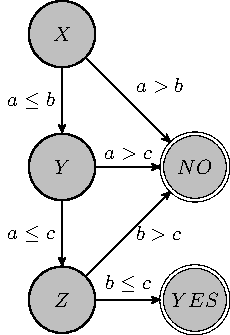
\includegraphics[width=0.28\textwidth,natwidth=\linewidth]{tikzfigs-figure0.pdf}
\caption{Control Flow Graph of \emph{isSorted(a, b, c)} \label{fig_cgf_example}}
\end{figure}

Figure \ref{fig:normal_concolic} shows an execution of the standard concolic testing algorithm on \emph{isSorted(a, b, c)}. A standard concolic tester starts from an arbitrary input ($[0, 0, 0]$ in this case), executes the UUT using the input values. The concolic tester collects the execution trace of this concrete execution and generates the path constraint $\pi_0 = [a \leq b, a \leq c, b \leq c]$. The last condition of $\pi_0$ is negated and we get $\pi_1 = [a \leq b, a \leq c, b > c]$. We invoke the constraint solver with $\pi_1$, denoted as CS(3), where 3 represents the number of path conditions in $\pi_1$. We get $[0, 1, 0]$ as the new input from the constraint solver. We execute the program with new inputs and collect the path constraint $\pi_2 = [a \leq b, a \leq c, b > c]$. Now, we negate the second condition of $\pi_2$ and remove all conditions after the second condition and get $\pi_3 = [a \leq b, a > c]$. We explain the reasons to exclude path conditions that come after the negated condition in Section \ref{subsec:ippc_alg_design}. We get $[0, 1, -1]$ by invoking CS(2). Concrete execution of the program results in $\pi_4 = [a \leq b, a > c]$. Then, we negate the only remaining path condition and get $\pi_5 = [a > b]$ after removing the last condition. CS(1) generates $[2, 1, -1]$. The concolic tester stops generating test inputs after executing the program since the resulting path constraint $\pi_6 = [a > b]$ has no path condition that is not negated before. At the end, we have invoked the constraint solver three times with an average path constraint length of two.

\begin{figure}[!t]
\begin{align*}
	i_1 & = [0, 0, 0] & [\text{initial inputs}] \\
	\pi_0 & = [a \leq b, a \leq c, b \leq c] & [\text{collected}]\\
	\pi_1 & = [a \leq b, a \leq c, b > c] & [\text{generated}]\\
	i_{2} & = [0, 1, 0] & [\text{CS(3)}] \\
	\pi_2 & = [a \leq b, a \leq c, b > c] & [\text{collected}] \\
	\pi_3 & = [a \leq b, a > c] & [\text{generated}]\\
	i_{3} & = [0, 1, -1] & [\text{CS(2)}] \\
	\pi_4 & = [a \leq b, a > c] & [\text{collected}] \\
	\pi_5 & = [a > b] & [\text{generated}] \\
	i_{4} & = [2, 1, -1] & [\text{CS(1)}] \\
	\pi_6 & = [a > b] & [\text{collected}] \\
	& \text{STOP} & [\text{Path Exhaustion}]
\end{align*}
\caption{A Sample Execution of Standard Concolic Testing on \emph{isSorted(a, b, c)}}
\label{fig:normal_concolic}
\end{figure}

\begin{figure}[!t]
\begin{align*}
	i_1 & = [0, 0, 0] & [\text{initial inputs}] \\
	\pi_0 & = [a \leq b, a \leq c, b \leq c] & [\text{collected}] \\
	\pi_1 & = [a \leq b, a \leq c, b > c] & [\text{generated}] \\
	\phi_1^0 & = [b > c] & [\text{overapproximation}] \\
	i_{2} & = [0, 1, 0] & [\text{CS(1)}] \\
	i_{2} & \text{~satisfies~} \pi_1 & CONTINUE \\
	\pi_2 & = [a \leq b, a \leq c, b > c] & [\text{collected}] \\
	\pi_3 & = [a \leq b, a > c] & [\text{generated}]\\
	\phi_3^0 & = [a > c] & [\text{overapproximation}] \\
	i_{3} & = [1, 1, 0] & [\text{CS(1)}] \\
	i_{3} & \text{~satisfies~} \pi_3 & CONTINUE \\
	\pi_4 & = [a \leq b, a > c] & [\text{collected}] \\
	\pi_5 & = [a > b] & [\text{generated}] \\
	\phi_5^0 & = [a > b] & [\text{overapproximation}] \\
	i_{4} & = [2, 1, 0] & [\text{CS(1)}] \\
	i_{4} & \text{~satisfies~} \pi_5 & CONTINUE \\
	\pi_6 & = [a > b] & [\text{collected}] \\
	& \text{STOP} & [\text{Path Exhaustion}]
\end{align*}
\caption{A Sample Execution of IPPC on \emph{isSorted(a, b, c)}}
\label{fig:ippc_concolic}
\end{figure}

Figure \ref{fig:ippc_concolic} illustrates the execution of our IPPC algorithm on \emph{isSorted(a, b ,c)}. In this case, each time we generate a new path constraint, we do not immediately call the constraint solver. We define the constraint obtained by executing the program a \emph{full path constraint}. We generate a subset of the full path constraint, $\phi^0$, which we call a \emph{partial path constraint}. Partial path constraint $\phi^0$ is initialized as an array which contains only the negated path condition. Partial path constraint generation phase is called \emph{overapproximation}. We call the constraint solver with $\phi^0$. In case  the constraint solver does not generate an input which satisfies $\pi$, we add the remaining path conditions of $\pi$ to $\phi^0$ and generate larger path constraints such as $\phi^1$, $\phi^2$ etc. until the constraint solver generates an input that satisfies $\pi$. For our example, we only made three calls to the constraint solver with average constraint length of one.

\section{Related Work}
\label{sec:related}

The idea of incremental constraint solving for concolic testing is as old as concolic testing itself and suggested along with CUTE, one of the first concolic testing tools \cite{Sen:2005:CCU:1095430.1081750}. However their incremental solving idea should not be confused with the one that we present in this paper. In CUTE, since they negate only one path condition, they keep the variables which are irrelevant to that path condition fixed. Therefore, they solve for variables which are only relevant to the negated path condition and decrease the burden on the constraint solver \cite{Sen:2005:CCU:1095430.1081750}. In our approach, CREST still does the incremental solving optimization of CUTE. On top of that, we also produce path contraints with fewer path conditions than a standard concolic tester.

Solving only a subset of path conditions instead of the whole path constraint is an approach recently used in finding integer overflows \cite{DBLP:conf/asplos/Sidiroglou-Douskos15}. The motivation is supported by observing that many of the path conditions of an execution trace are irrelevant w.r.t. integer overflows. In our work, we make a more general assumption that some of the path conditions should be irrelevant to the execution trace itself. Experimental results support our motivational assumption.

All concolic testers require a \emph{constraint solver}. Z3 and Yices are commonly used constraint solvers \cite{Yices, DeMoura:2008:ZES:1792734.1792766}. Details on the complexity of constraint solving can be found in \cite{Tsang93foundationsof}. Standard constraint solvers are not able to solve all types of constraints \cite{Qu:2011:CSC:2082758.2083418}. There are constraint solvers which solve nonlinear constraints \cite{Nuzzo:2010:CSS:1998496.1998513} and constraint solvers which solve constraints involving high-precision rational numbers \cite{Souza:2011:CSC:1986308.1986337}. Yun et al. has modified CREST to use Z3 constraint solver in order to support nonlinear arithmetic \cite{website:crestz3}. We could easily implement IPPC modification on top CREST-z3, although plain CREST is sufficient for our experiments.

Concolic testing is not restricted to sequential programs. There are concolic testers which test concurrent software \cite{Farzan:2013:CT:2491411.2491453}. Therefore, IPPC can also be used to test concurrent units.

Many concolic testers (e.g. CUTE) use bounded depth first search (\emph{bDFS}) instead of bounding the number of iterations as in IPPC and CREST \cite{Sen:2005:CCU:1095430.1081750, Sen:2006:Thesis}. \emph{bDFS} can be viewed as an attempt to keep the number of path conditions limited. We believe that our approach makes bounding the number of iterations more preferable to bounding the depth of the search as in \emph{bDFS} since experiments show that IPPC already reduces the size of path constraints significantly.

\emph{Random branch selection (RND)} is an approach introduced in CREST \cite{Burnim:2008:HSD:1642931.1642995}. In random branch selection one negates each path condition of a path constraint with probability $0.5$. A variant of this strategy negates only one path condition at random and calls the constraint solver with that path condition.

\emph{Control flow directed search (CFG)} is a search strategy which guides the search using the static structure of the UUT. CFG assigns weights to edges of the control flow graph of the UUT and calculates distances to each unvisited branch. Then, CFG solves a path constraint which leads to the unvisited branch with the least distance to the current execution trace \cite{Burnim:2008:HSD:1642931.1642995}. We compare our approach with both CFG and RND.

A recent study on CREST proposes a new search strategy, called DYNASTY, which uses the control flow graph of the UUT to guide the search as in CFG technique \cite{Dong:2011:AHB:2056316.2057002}. They modify CREST as in our work and increase branch coverage with fewer iterations. Their approach is based on avoiding infeasible paths, whereas our approach decreases the penalty of hitting an infeasible path by using partial path constraints.

\section{Incremental Partial Path Constraint (IPPC)}
\label{sec:ppc}

In this section, we describe IPPC in detail. % and caching optimizations.

\subsection{Background}

We have previously stated that a concolic tester generates path conditions from an execution trace of the UUT. We define the following using this fact:

\theoremstyle{definition}
\newtheorem{definition}{Definition}

\theoremstyle{plain}
\newtheorem{axiom}{Axiom}
\newtheorem{theorem}{Theorem}
\begin{definition}
A \emph{path condition} is a function of symbolic variables to $\lbrace T, F \rbrace$.
\end{definition}

\begin{definition}
An \emph{input vector} is an assignment to all symbolic variables of UUT.
\end{definition}

\begin{definition}
A \emph{full path constraint} is an array whose elements form a set of path conditions. 
\end{definition}

\begin{definition}
Any array whose elements form a subset of the elements of the full path constraint is called a \emph{partial path constraint}.
\end{definition}

\begin{definition}
An input vector is said to $satisfy$ a path constraint if and only if the input vector makes all conditions of the path constraint $T$.
\end{definition}

Conjunction of all conditions in a partial path constraint is an overapproximation of conjunction of all conditions in the full path constraint. Therefore the process of generating partial path constraints from full path constraints is called an \emph{overapproximation}.

\begin{definition}
An algorithm which takes a path constraint and returns an input vector which satisfies that constraint is called a \emph{constraint solver}. If there exists no such input vector, it returns \emph{null}.
\end{definition}

We used the Yices constraint solver, which is the default solver in CREST \cite{Yices, Burnim:2008:HSD:1642931.1642995}.

%\begin{axiom}
%\label{axiom:determinism}
%All input vectors which satisfy the full path constraint must generate the same execution trace.
%\end{axiom}
%
%Axiom \ref{axiom:determinism} assumes that the given UUT is \emph{deterministic}.

\subsection{Algorithm Design of IPPC}
\label{subsec:ippc_alg_design}

We implemented IPPC on top of CREST's standard concolic testing algorithm (denoted by DFS) as shown in Algorithm \ref{fig_concolic_alg}. We initially give $\emph{nIterations} \leftarrow 0$, $\emph{TestInput} \leftarrow \emph{random\_input}$ and $\emph{TestInputs} \leftarrow \emptyset$. We can see from line 1 that the algorithm is bounded by the maximum number of iterations. At line 2, we check the input vector because constraint solver is assumed to return \emph{null} if an input vector can not be generated, i.e. given path constraint is infeasible. We increment iterations only if the path constraint is satisfiable. At line 4, we execute $UUT$ with $input$ and save the full path constraint of the execution trace as $\pi$. Lines 8 and 9 ensure that the algorithm performs a depth first search (DFS). We always negate the last unvisited condition of a path constraint. If there exists no path condition that is not negated before, we stop because all paths are executed. At line 11, constraintSolver takes a path constraint and returns a satisfying input vector. We don't terminate the solver, we use it in it's built-in incremental mode. Notice that we exclude the path conditions which come after the negated path condition. Any input vector which satisfies path conditions up to the negated path condition must generate the same execution trace up to the occurrence of the negated path condition. Negated path condition will force the program to a different execution trace. So, path conditions coming after the negated condition is not a part of the new execution trace and therefore should be removed. If the unnecessary path conditions are not excluded, they may cause false path constraint infeasibilities. False infeasibilities force the concolic tester not to generate any input vector for the path constraint and therefore cause a decrease in test coverage.

\begin{algorithm}[!t]
\SetKwData{Out}{testInputs}\SetKwData{NITR}{nIterations}\SetKwData{TestInput}{testInput}\SetKwData{UUT}{uut}\SetKwData{MaxItr}{maxIterations}\SetKwData{Null}{\textbf{null}}\SetKwData{Pi}{$\pi$}\SetKwData{I}{i}
\SetKw{KwGoTo}{goto}\SetKw{KwReturn}{return}
\SetKwFunction{RndVector}{generateRandomInputVector}\SetKwFunction{Execute}{execute}\SetKwFunction{Add}{add}\SetKwFunction{SizeOf}{sizeOf}\SetKwFunction{IsNegatedBefore}{isNegatedBefore}\SetKwFunction{SetNegatedBefore}{setNegatedBefore}\SetKwFunction{CS}{constraintSolver}\SetKwFunction{DFS}{crest}
\SetKwInOut{Input}{input}\SetKwInOut{Output}{output}
\Input{uut (unit under test)\\maxIterations\\testInput\\testInputs\\nIterations}
\Output{testInputs}
\BlankLine
%\Out$\leftarrow \emptyset$\;
%\J$\leftarrow 0$\;
%\TestInput$\leftarrow$ \RndVector{}\;
	\If{\NITR $<$ \MaxItr}
		{\label{Line4}
			\If{\TestInput $\neq$ \Null}
				{
					\NITR$\leftarrow$\NITR$+1$\;
					\Pi$\leftarrow$\Execute{\UUT, \TestInput}\;
					\Add{\Out, \TestInput}\;
				}
			\For{\I$\leftarrow $\SizeOf{\Pi}$-1$ \KwTo $0$}
				{
					\If{$!$\IsNegatedBefore{$\Pi[\I]$}}
						{
							\SetNegatedBefore{$\Pi[\I]$}\;
							$\Pi[\I] \leftarrow \neg \Pi[\I]$\;
							\TestInput$\leftarrow$ \CS{$\lbrace \Pi[0]...\Pi[i] \rbrace$}\;
							\KwReturn \DFS{\UUT, \MaxItr, \TestInput, \Out, \NITR}\;
							%\KwGoTo \ref{Line4}\;
						}
				}
		}
\KwReturn \Out\;

\caption{Concolic Testing Algorithm Implementing DFS with Maximum Iterations (CREST)} \label{fig_concolic_alg}
\end{algorithm}

IPPC is exactly the same as Algorithm \ref{fig_concolic_alg} except we replace line 11 with 
$input \leftarrow $ IPPC\_Solve $(UUT, \lbrace\pi[0]...\pi[i]\rbrace, \lbrace\pi[i]\rbrace)$. We describe IPPC\_Solve in Algorithm \ref{fig_ippc_alg}. We keep the solver running in incremental mode.

Line 1 of Algorithm \ref{fig_ippc_alg} invokes the constraint solver with $\phi$. If the constraint solver is unable to generate an input vector, we conclude that the full path constraint is also \emph{infeasible} and return \emph{null}. We prove the infeasiblity of a full path constraint given the infeasibility of a partial path constraint in Theorem \ref{thm:infeasibility}. The for loop starting at line 5 checks if the input vector satisfies the full path constraint. If $input$ satisfies $\pi$, we can return $input$. If not, we \emph{learn} the unsatisfied path condition by adding it to $\phi$ and generate a new input vector. This process may be continued until $\phi = \pi$ in the worst case where either an input can be generated or $\pi$ is infeasible given that the constraint solver is sound (if exists, returns a correct test input) and complete (terminates and is correct for all cases). This worst case condition is rare or non existent at least in our experiments.

\begin{algorithm}
\SetKwData{TestInput}{testInput}\SetKwData{UUT}{uut}\SetKwData{MaxItr}{maxIterations}\SetKwData{Null}{\textbf{null}}\SetKwData{Pi}{$\pi$}\SetKwData{I}{i}\SetKwData{PPC}{$\phi$}
\SetKw{KwGoTo}{goto}\SetKw{KwReturn}{return}
\SetKwFunction{Append}{append}\SetKwFunction{Add}{add}\SetKwFunction{SizeOf}{sizeOf}\SetKwFunction{CS}{constraintSolver}\SetKwFunction{SAT}{sat}\SetKwFunction{IPPC}{IPPC\_Solve}
\SetKwInOut{Input}{input}\SetKwInOut{Output}{output}
\Input{uut (unit under test)\\$\pi$ (full path constraint)\\$\phi$ (partial path constraint)}
\Output{testInput}
\BlankLine
%\PPC$\leftarrow \lbrace \Pi[\SizeOf{\Pi}-1] \rbrace$\;
\TestInput$\leftarrow \CS{\PPC}$\;\label{Line2}
	\If{\TestInput $=$ \Null}
		{
			\KwReturn \Null\;
		}
	\For{\I$\leftarrow 0$ \KwTo $\SizeOf{\Pi} - 1$}
		{
			\If{$!$\SAT{$\TestInput, \Pi[\I]$}}
				{
					\Append{$\PPC, \Pi[\I]$}\;
					\KwReturn \IPPC(uut, \Pi, \PPC)\;
					%\KwGoTo \ref{Line2}\;
				}
		}
\KwReturn \TestInput\;
\caption{IPPC\_Solve} \label{fig_ippc_alg}
\end{algorithm}

\subsection{Correctness and Completeness}

To be able to produce readable proofs, we assume all boolean operations on a path constraint are performed on the conjunction of all conditions of the path constraint.

\begin{theorem}
\label{thm:infeasibility}
If a partial path constraint $\phi$ is unsatisfiable, then its full path constraint $\pi$ is also unsatisfiable.
\end{theorem}

\begin{proof}
Since $\phi$ is unsatisfiable, $\neg \phi$ is valid. Since $\phi$ is an overapproximation of $\pi$, $\pi \rightarrow \phi$ by definition. Therefore by modus tollens, $\neg \pi$ is valid. In other words, $\pi$ is unsatisfiable.
\end{proof}

We now show the correctness of IPPC\_Solve. We change only one line in Algorithm \ref{fig_concolic_alg}. Therefore, to prove the correctness of IPPC, we only need to ensure that for all path constraints, IPPC\_Solve generates an input vector that has the same property as the input vector generated by the constraint solver. If such an input vector exists, a constraint solver always generates an input vector that satisfies the full path constraint.

\begin{theorem}
\label{thm:correctness}
(a) IPPC\_Solve generates \emph{null} whenever the constraint solver in Algorithm \ref{fig_concolic_alg} at Line 11 generates \emph{null}. (b) Otherwise IPPC\_Solve always generates an input vector that satisfies the full path constraint.
\end{theorem}

\begin{proof}
Proof of (a) is trivial due to lines 1-4 of Algorithm \ref{fig_ippc_alg}. We can see from lines 5-10, that Algorithm \ref{fig_ippc_alg} would not stop until the input vector satisfies the full path constraint. Therefore proof of (b) is trivial as well.
\end{proof}

\begin{theorem}
\label{thm:completeness}
IPPC\_Solve is correct and eventually terminates, i.e. IPPC\_Solve is complete.
\end{theorem}

\begin{proof}
IPPC\_Solve is correct by Theorem \ref{thm:correctness}. The second part of the proof is as follows. At any time, partial path constraint $\phi$ is either (a) unsatisfiable, or an input vector $i$ is generated. If an input vector $i$ is generated, either (b) $i$ satisfies $\pi$, or (c) we add a new path condition of full path constraint to $\phi$. If (a), IPPC\_Solve returns \emph{null} and terminates. If (b), IPPC\_Solve returns $i$ and terminates. If (c) happens $N-1$ times, where $N$ denotes the number of path conditions in $\pi$, $\phi \leftrightarrow \pi$ must hold. In other words, we build up the partial path constraint up to the full path constraint. In that case, the constraint solver must either generate \emph{null} or generate a satisfying input vector, therefore the algorithm terminates.
\end{proof}

\begin{table}
\centering
\caption{List of Benchmarks}
\vspace*{2pt}
\begin{tabular}{|c|cc|}
\hline
\textbf{UUT} & \textbf{KLOC} & \textbf{{\#}vars} \\
\hline
gcd & 0.05 & 2 \\ 
bsort & 0.05 & 30 \\
sqrt & 0.06 & 1 \\
prime & 0.1 & 1 \\
factor & 0.2 & 1 \\
replace & 0.5 & 20 \\
ptokens & 0.6 & 40 \\
grep & 15 & 10 \\
\hline
\end{tabular}
\label{tbl:benchmarks}
\end{table}


\begin{table*}
\setlength{\tabcolsep}{3pt}
\centering
%\vspace*{2pt}
\caption{Experimental Results (Best results are highlighted)}
\begin{scriptsize}
%\hspace*{-10pt}
\begin{tabular}{|c|c|cccc|cccc|cccc|cccc|}
\hline
\multirow{2}{*}{\begin{scriptsize}\textbf{UUT}\end{scriptsize}}        & \multirow{2}{*}{\begin{scriptsize}\textbf{\#Itr}\end{scriptsize}} & \multicolumn{4}{c|}{\begin{scriptsize}\textbf{Total CS Calls}\end{scriptsize}} & \multicolumn{4}{c|}{\begin{scriptsize}\textbf{Avg Const. Size}\end{scriptsize}} & \multicolumn{4}{c|}{\begin{scriptsize}\textbf{Branch Coverage (\%)}\end{scriptsize}} & \multicolumn{4}{c|}{\begin{scriptsize}\textbf{Time Elapsed (sec)}\end{scriptsize}} \\
                            &                         & DFS    & CFG    & RND    & IPPC    & DFS     & CFG    & RND    & IPPC    & DFS     & CFG    & RND    & IPPC    & DFS      & CFG      & RND     & IPPC    \\
\hline
\multirow{3}{*}{gcd}        &             1000            &   5681     &   866     &   1105     &   11004      &   161.0      &   4.1     &   2.9     &   1.9      &   100      &   100     &   100     &    100     &   22.6       &    5.7      &   \textbf{3.9}      &    7.5      \\
                            &          5000               &    25801    &    4364    &   5653     &   64844      &   188.6      &   5.7     &   2.8     &   1.9      &    100     &   100     &   100     &    100    &    119.5      &    24.8      &   \textbf{21.6}      &   34.7    \\
                            &         10000                &   47367     &    8761    &   11287     &    120678     &    206.3     &   5.9     &   2.8     &    1.9      &    100     &   100     &   100     &   100      &   234.5       &    48.7      &   \textbf{45.7}      &     125.5     \\
\hline
\multirow{3}{*}{bsort} &         100                &   117     &   53     &   104     &    1346     &    145.7     &   148.5     &    88.9    &    10.3     &    100      &   100     &   100     &   100      &    1.1      &    \textbf{0.8}      &    0.9     &    1.3      \\
                            &          500               &    711    &   284     &    537    &    10306     &    308.9     &   165.3     &   115.5     &   12.7      &     100    &   100     &   100     &   100      &    7.6      &    5.0      &    \textbf{4.8}     &     9.2       \\
                            &          1000               &    1462    &   571     &   1063     &   25023      &    342.5     &   165.0     &   132.6     &    14.3     &    100     &   100     &   100     &    100     &    15.5      &     \textbf{8.7}     &    9.5     &    21.9      \\
\hline
\multirow{3}{*}{sqrt} &         1000                &   1010     &   980     &   1064     &    1006     &    17.2     &   2.3     &    1.8    &    1.0     &    94.4      &   94.4     &   94.4     &   94.4      &    4.3      &    4.5      &    4.3     &    \textbf{3.9}      \\
                            &          5000               &    5001    &   4894     &    5372    &    5006     &    24.0    &   2.3     &   1.8     &   1.0      &     94.4      &   94.4     &   94.4     &   94.4      &    30.1      &    23.1      &    22.2     &     \textbf{20.3}       \\
                            &          10000               &    10010    &   9820     &   10732     &   10014      &    22.7     &   2.3     &   1.8     &    1.0     &    94.4      &   94.4     &   94.4     &   94.4     &    45.9      &     42.0     &    42.2     &    \textbf{39.1}      \\
\hline
\multirow{3}{*}{prime}      &         100                &   1275     &   92     &   111     &    132     &    103.3     &   7.5     &   4.8     &    1.2     &    \textbf{92.5}     &   85     &   62.5     &   \textbf{92.5}    &    2.3      &    0.5      &    0.5     &    \textbf{0.4}      \\
                            &         175                &    3946    &    165    &    212    &    253     &    186.6     &    8.0    &   4.0     &    1.2     &    \textbf{92.5}     &   90     &    70    &   \textbf{92.5}      &    10.1      &    1.0      &    1.1     &    \textbf{0.8}      \\
                            &          250               &   4166     &    236    &    287    &    1688     &    189.6     &    7.2    &   4.1     &   1.8      &    \textbf{92.5}     &     92.5   &   82.5     &    \textbf{92.5}     &    13.5      &    1.6      &   1.6      &    \textbf{1.5}      \\
\hline
\multirow{3}{*}{factor}     &        50                 &    2678    &    80    &    110    &    7693     &    222.1     &    2.9    &   4.0     &    1.9     &    \textbf{94.2}     &   \textbf{94.2}     &   76.9     &   \textbf{94.2}      &    8.6      &     \textbf{0.2}     &    \textbf{0.2}     &    1.5      \\
                            &          75               &    5734    &    111    &    145    &    25255     &    249.7     &   3.4     &   4.7     &   1.9      &    \textbf{94.2}     &   \textbf{94.2}     &   83.2     &    \textbf{94.2}     &     23.5     &    \textbf{0.3}      &    \textbf{0.3}     &    4.6      \\
                            &          100               &   11157     &   148     &    243    &    34218     &    310.9     &    2.8    &   16.0     &    1.9     &   \textbf{94.2}      &   \textbf{94.2}     &   89.4     &    \textbf{94.2}     &    120.3      &    0.6      &    \textbf{0.5}     &    6.4      \\
\hline
\multirow{3}{*}{replace}    &          1000               &   1129     &   1024     &    1024    &    6847     &   16.6      &    25.9    &   31.7     &    3.8     &    85.2     &    \textbf{88.7}    &    85.2    &   85.2      &   \textbf{4.1}       &     4.5     &    \textbf{4.1}     &    5.8      \\
                            &         5000                &   5623     &    5193    &   5167     &    43695     &    21.5     &   28.4     &   32.4     &    4.8     &            88.7     &   \textbf{90.8}     &     88.7   &   88.7       &     \textbf{22.0}     &    23.8     &   22.4   &  31.4  \\
                            &         10000               &    10936    &    10270    &    10301    &    103590     &    24.5     &    28.0    &    33.0    &     5.6    &           88.7     &    \textbf{90.8}    &    90.8     &    88.7      &     \textbf{43.1}     &    45.5     &   44.6   &  66.9  \\
\hline
\multirow{3}{*}{ptokens}    &          1000               &   1181     &   1355     &    1319    &    38415     &   591.0      &    136.8    &   102.2    &    29.8     &    \textbf{85.1}     &   79.8   &    79.8    &   \textbf{85.1}      &   30.0       &     9.4     &    \textbf{8.6}     &    18.5      \\
                            &         5000                &   6394     &    6976    &   6739     &    253829     &    1949.9      &   148.7     &    103.2     &    37.5   & \textbf{85.1}     &     84.4     &     84.9   &   \textbf{85.1}       &     212.4     &    48.4     &   \textbf{47.7}   &  106.1  \\
                            &         10000               &    13394    &    13838    &    13510    &    432262     &    2241.6     &    163.7    &    99.7    &     30.5    &    \textbf{91.5}    &    89.6    &    88.9     &    \textbf{91.5}      &     321.7     &    106.8     &   \textbf{91.2}   &  210.8  \\
\hline
\multirow{3}{*}{grep}       &          100               &    100    &   N/A     &   121     &    436     &    59.0     &    N/A    &    362.0    &    3.2     &  16.7    &    N/A    &    16.7    &    16.7     &     \textbf{0.3}     &     N/A     &    0.4     &    0.4      \\
                            &          220               &    269    &   N/A     &   272     &    1671     &    178.4     &   N/A     &   332.2     &    4.7     &    16.7     &    N/A    &    16.7    &    16.7     &     \textbf{0.9}     &     N/A     &    \textbf{0.9}    &     1.0     \\
                            &          340               &    439    &   N/A     &   451     &    3671     &    324.8     &   N/A     &    350.1    &    8.3     &    16.7     &    N/A    &     16.7   &     16.7    &     1.6     &     N/A     &    \textbf{1.5}     &    1.9     \\
\hline
\end{tabular}\label{tbl:allresults}
\end{scriptsize}

\end{table*}

\section{Experimental Study}
\label{sec:experiments}

We implemented IPPC on top of CREST tool. Our implementation of IPPC and experimental results are available online \cite{website:crestppc}. CREST implements the standard concolic testing algorithm (DFS) and two different improvements, denoted by CFG and RND. We compared IPPC with these three techniques. Techniques we used in experiments are as follows.
%\emph{http://bitbucket.org/yavuzkoroglu/crest-ppc} to reproduce the experiments. 

\begin{enumerate}
\item \textbf{DFS:} Standard concolic testing algorithm.
\item \textbf{CFG:} Control flow directed testing algorithm. 
\item \textbf{RND:} Random branch testing heuristic on top of the standard concolic testing algorithm.
\item \textbf{IPPC:} Our Incremental Partial Path Constraint algorithm.
\end{enumerate}

Brief explanations of CFG and RND algorithms are given in Section \ref{sec:related}.

We carried out the experiments on a virtual Linux guest with 1024MB memory and one CPU hosted by a MacBook Pro with an Intel Core i7 2.9 GHz GPU and 8GB Memory. We collected the following information for each experiment:

\begin{enumerate}
\item \textbf{Time elapsed:} Time spent to test the UUT.
\item \textbf{Total CS Calls:} Total number of constraint solver calls made by the concolic tester.
\item \textbf{Avg Const. Size:} Average size of path constraints solved by the constraint solver. 
%\item \textbf{Max Constraint Size:} Maximum size of path constraints solved by the constraint solver. 
%\item \textbf{Number of Tests:} Number of different input vectors generated by the concolic tester. 
\item \textbf{Branch Coverage:} Measurement of total branch coverage of UUT. %We have implemented a script which uses \texttt{GNU gcov} to measure branch coverage for each case. 
\end{enumerate}

Concolic testing involves a degree of randomness due to the randomness of initial inputs. Therefore we performed 10 executions of each experiment and took average values of each measure. All of our experimental results can be found in Table \ref{tbl:allresults}.

Table \ref{tbl:benchmarks} shows the program units we used in our experiments. Column \emph{KLOC} represents the lines of code measured in thousands. Column \emph{{\#}vars} represents the number of symbolic variables.

We implemented five small benchmarks, \emph{gcd}, \emph{bsort}, \emph{sqrt}, \emph{prime} and \emph{factor} to conduct our initial experiments. \emph{gcd} implements the binary greatest common divisor algorithm. We downloaded and modified the bubble sort algorithm \emph{bsort}, which sorts a given array of integers \cite{website:bubblesort}. \emph{sqrt} takes the floor of the square root of a given integer. \emph{prime} decides whether a given integer is prime or not. \emph{factor} is an integer factorization algorithm. \emph{replace} and \emph{grep} are benchmarks that come with CREST framework and used in several research studies on concolic testing \cite{Burnim:2008:HSD:1642931.1642995, Dong:2011:AHB:2056316.2057002, Seo:2014}. \emph{ptokens} is the printtokens  benchmark available at Software Infrastructure Repository (SIR) \cite{SIR}. \emph{ptokens} tokenizes the given string according to a grammar. For reasons described in Section \ref{subsec:threats}, our implementation of \emph{gcd}, \emph{prime} and \emph{factor} do not contain any bitwise masking or modulo operations. Instead, we decide divisibility via only subtraction and comparison operations. Also, \emph{sqrt} does not use any floating point operations since CREST has no symbolic equivalent of floating point variables.

In our experiments, we used programs in different sizes. None of the given programs are too large in size so they can be tested in reasonable time without getting into scalability issues. In our experimental set, we argue that the structure of UUT is related to the performance of the testers that we use rather than the sizes of the programs. We observed that small programs such as \emph{factor} can have very long runtimes (120 sec). We argue that IPPC will perform well not when the program is small or large, but when the program contains many infeasible paths. Although being small, \emph{prime} and \emph{factor} contain many infeasible paths. Although being large, \emph{grep} and \emph{replace} did not contain many infeasible paths.

We show all experimental results in Table \ref{tbl:allresults}. CFG method is not applicable to \emph{grep} due to a bug in CREST, therefore we used \emph{N/A} to denote the results we could not observe. We used 1000, 5000 and 10000 as the maximum number of iterations (\emph{{\#}Itr}) in experiments. We decreased \emph{{\#}Itr} for \emph{prime}, \emph{factor}, \emph{bsort} and \emph{grep}, since those units have few distinct execution traces. When there are few distinct execution traces and \emph{{\#}Itr} is too high, DFS and IPPC are able to stop before completing \emph{{\#}Itr} iterations, since they check if all execution traces are explored or not. However, CFG and RND have no such stopping condition and iterate \emph{{\#}Itr} times. So, if we kept \emph{{\#}Itr} high for \emph{prime}, \emph{factor}, \emph{bsort} and \emph{grep}, it would unfairly result in bad runtimes for CFG and RND.

%\begin{table}
%\centering
%\caption{Best Speedups}
%\label{tbl:bestspeeds}
%\begin{tabular}{|c|cccc|}
%\hline
%       & DFS & CFG & RND & IPPC \\
%\hline
%DFS &   1x        &  1.09x &  1.33x & 1.55x \\
%CFG &   200.5x &     1x   &  1.125x & 10.6x \\
%RND &   240.6x &  1.46x &     1x    & 12.8x \\
%IPPC & 18.79x &  1.25x & 1.375x &   1x\\
%\hline
%\end{tabular}
%\end{table}

We show the best algorithms for each benchmark in Table \ref{tbl:bestres} where \emph{All Equal} means all techniques are equally well. The column denoted as \emph{by Runtime First} compares techniques by runtime first, if techniques have similar runtimes, compares branch coverages. The last column compares techniques by coverage first. 
DFS does not perform well in both columns. In terms of runtimes RND is the best and IPPC is the second. In terms of coverage CFG and IPPC are the best.
Hence, IPPC performs well in both categories.
%IPPC dominates all other techniques in two of the eight cases in both columns. IPPC has the best coverage levels in three of the experiments. 


\begin{table}
\centering
\caption{Best Concolic Testers}
\vspace*{3pt}
\label{tbl:bestres}
\begin{tabular}{|c|cc|}
\hline
\textbf{UUT} & \textbf{by Runtime First} & \textbf{by Coverage First} \\
\hline
gcd & RND & RND \\
bsort & CFG & CFG \\
sqrt & IPPC & IPPC{\&}DFS \\
prime & IPPC & IPPC{\&}DFS \\
factor & RND & CFG \\
replace & DFS & CFG \\
ptokens & RND & IPPC \\
grep & All Equal & All Equal \\
\hline
\end{tabular}
\end{table}

%We obtain the following results by observing \emph{Time Elapsed (sec)} column of Table \ref{tbl:allresults}. IPPC is faster than DFS in five of eight experiments. 

We next compare IPPC with DFS in more detail since IPPC is derived from DFS.
%
We observe from Table \ref{tbl:speedup} that there exists a correlation between Avg Const. Size of DFS / Avg Const. Size of IPPC and speedup of IPPC over DFS. When the gap between the constraint sizes of DFS and IPPC increases, the speedup of IPPC over DFS increases with the slight exception of \emph{grep}.
Similarly, Figure \ref{fig:speedup} shows that whenever the number of constraint solver calls (Total CS Calls) of DFS is close to the maximum number of iterations ({\#}Itr), DFS works faster. If DFS makes many more calls than the number of iterations, IPPC works faster. Normally, DFS is expected to call constraint solver exactly once for each iteration. DFS makes more than one constraint solver call for an iteration only if the generated path constraint for that iteration is infeasible. In that case, DFS changes the path constraint and calls constraint solver repeatedly until a feasible path is found. We believe \emph{factor} has the largest number of infeasibilities since DFS makes many constraint solver calls for few iterations. Figure \ref{fig:speedup} shows that the speedup of IPPC over DFS is above 5x when DFS generates four or more infeasible path constraints for each feasible path constraint (i.e. DFS makes more than five constraint solver calls for each iteration, $\text{{\#}Itr} / \text{Total CS Calls of DFS} < 0.2$). Therefore, IPPC finds infeasibilities faster for all benchmarks.

%\begin{table}[!t]
%\centering
%\caption{IPPC Speedup over DFS}
%\label{tbl:speedup}
%\begin{tabular}{|c|cc|}
%\hline
%\multirow{2}{*}{\textbf{UUT}} & Avg Const. Size Ratio & Speedup \\
%                                              & (DFS / IPPC) & ($t_{\text{DFS}} / t_{\text{IPPC}}$) \\
%\hline
%replace & 4.4 & 0.6x \\
%bsort & 20.8 & 0.79x \\
%sqrt & 21.3 & 1.25x \\
%grep & 31.8 & 0.83x \\
%ptokens & 48.4 & 1.7x \\
%gcd & 97.5 & 2.77x \\
%prime & 115.6 & 9.1x \\
%factor & 137.3 & 9.8x \\
%\hline
%\end{tabular}
%\end{table}

\begin{figure}
\centering
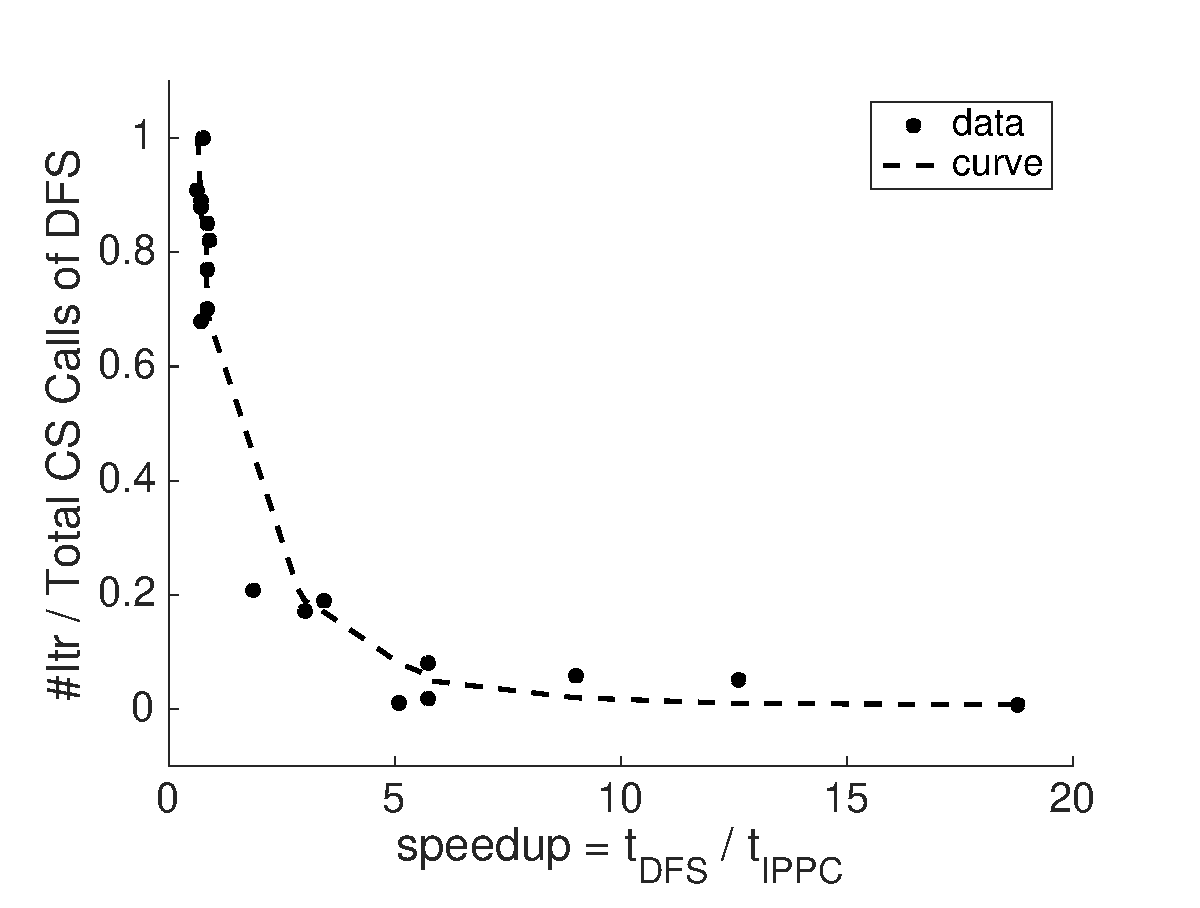
\includegraphics[width=0.42\textwidth]{speedup}
\qquad
\setlength{\tabcolsep}{3pt}
\begin{tabular}[b]{|c|cc|}
\hline
\multirow{2}{*}{\textbf{UUT}} & Avg Const. Size Ratio & Speedup \\
                                              & (DFS / IPPC) & ($t_{\text{DFS}} / t_{\text{IPPC}}$) \\
\hline
replace & 4.4 & 0.6x \\
bsort & 20.8 & 0.79x \\
sqrt & 21.3 & 1.25x \\
grep & 31.8 & 0.83x \\
ptokens & 48.4 & 1.7x \\
gcd & 97.5 & 2.77x \\
prime & 115.6 & 9.1x \\
factor & 137.3 & 9.8x \\
\hline
\end{tabular}
\captionlistentry[table]{Relationship between Speedup and {\#}Infeasible Constraints (Figure \ref{fig:speedup}) and IPPC Speedup over DFS (Table \ref{tbl:speedup}).}
\captionsetup{labelformat=andtable}
\caption{Relationship between Speedup and {\#}Infeasible Constraints (Figure \ref{fig:speedup}) and IPPC Speedup over DFS (Table \ref{tbl:speedup}).}\label{fig:speedup}\label{tbl:speedup}
\end{figure}

 % To support our claim, we consider pairwise best case speedups of each tecnique. Best speedups of all techniques are given in Table \ref{tbl:bestspeeds}. The table shows speedups of techniques at the rows over techniques at the columns (i.e. divides runtimes of techniques at the columns to techniques at the rows). From Table \ref{tbl:bestspeeds}, we can observe that each tecnique has a best case speedup over the other.

In all experiments, the largest path constraint produced by IPPC had a length of 157, whereas the largest path constraints of DFS, CFG and RND had lengths of 2922, 1603 and 1391, respectively. We conclude that we eliminated the need for solving large path constraints to generate test inputs while keeping the runtimes fast and coverage high using IPPC.

We get exactly the same coverage results for both IPPC and DFS. We expect this since both algorithms perform a depth-first search. We argue that the coverage results being similar indicates that IPPC correctly does DFS on the UUT while improving the performance.

IPPC considers constraints that are 10x smaller than other techniques. We believe it is because that IPPC finds infeasibilities early, since most infeasibilities arise from a combination of few conditions in the constraint.

%\begin{figure}
%\centering
%\includegraphics[width=\linewidth]{TimePrime}
%\caption{Runtimes of \emph{prime} Benchmark.}
%\label{fig:timeprime}
%\end{figure}
%
%\begin{figure}
%\centering
%\includegraphics[width=\linewidth]{CSCallsPrime}
%\caption{Total CS Calls of \emph{prime} Benchmark.}
%\label{fig:csprime}
%\end{figure}
%
%\begin{figure}
%\centering
%\includegraphics[width=\linewidth]{ConstSizePrime}
%\caption{Avg const. sizes of \emph{prime} Benchmark.}
%\label{fig:constszprime}
%\end{figure}
%
%\begin{figure}
%\centering
%\includegraphics[width=\linewidth]{BranchCovPrime}
%\caption{Coverages of \emph{prime} Benchmark.}
%\label{fig:brcovprime}
%\end{figure}


%Figure \ref{fig:timeprime} clearly indicates that IPPC performs better than standard concolic tester (DFS). Figures \ref{fig:csprime} and \ref{fig:constszprime} also indicate that IPPC decreases the burden of constraint solver significantly compared with other techniques. Notice that Figures \ref{fig:csprime} and \ref{fig:constszprime} are on logarithmic scale. Figure \ref{fig:brcovprime} indicates that we achieve good branch coverage levels compared with other techniques.

\section{Threads to Validity}
\label{subsec:threats}
We assume that the constraint solver is sound, i.e. the constraint solver can find an input vector whenever there exists an input vector which satisfies the path constraint. In general, this assumption is not valid. We know that the constraint solver used in CREST, Yices \cite{Yices, Qu:2011:CSC:2082758.2083418}, does not find solutions for nonlinear path conditions (e.g. $x_2 x_1 < 12$). We also know that CREST may not be able to solve conditions involving modulo operation and bitwise masking \cite{Qu:2011:CSC:2082758.2083418}. All path conditions generated in our experiments are linear, in other words they can be written as $k \bowtie \sum_{i=1}^{N} c_i x_i$ where $\bowtie \in \lbrace <, \leq, =, \neq, >, \geq \rbrace$, $k \in \mathrm{R}$, $\forall i \in \lbrace 1, ..., N \rbrace, c_i \in \mathrm{R}$ and $N$: total number of symbolic variables). All path conditions in our experiments are also free of modulo and bit masking operations. Hence, we safely assume that the constraint solver is sound in our environment. We also do not use any floating point arithmetic.

The UUT can have intermediary variables calculated from symbolic variables and therefore can have path conditions on those intermediary variables. All path conditions that CREST returns are on the initial symbolic variables. Therefore, even if all branch conditions in the code may seem trivial, CREST may fail to generate correct inputs if variables are nonlinear (e.g. multiplication of two symbolic variables).

We assume the UUT to be \emph{sequential} and \emph{deterministic}, i.e. if an input vector $i$ produces an execution trace $e$, $i$ will always produce $e$ for this UUT. However, for example a process which depends on random numbers could violate this assumption. We carefully chose the experiments so that we never violate these basic assumptions.

We assume the UUT is \emph{terminating}, since if UUT halts, so does the tester as well. The test cases we chose and the test cases in previous work are all terminating.

We report runtimes that we acquired from a virtual environment. We got similar results on an host machine as well.

It is possible that IPPC may learn partial path constraints up to a point that they become full path constraints. So in the worst case, a standard concolic tester is more efficient than IPPC. However, our experimental results show that we require only a small portion of the full path constraint to generate input vectors belonging to the same equivalence class, i.e. input vectors which generate same execution traces when given to UUT.

\section{Conclusions and Future Work}
\label{sec:conclusions}

In this paper, we designed a constraint solving strategy, called Incremental Partial Path Constraints (IPPC), which eliminates the need for solving large constraints to generate unit tests. We compared our design with other concolic testing algorithms in experiments. We observed that when there are many infeasible path constraints in a program, IPPC has more than 5x speedup over a standard concolic tester. We significantly reduce the number of path conditions required to generate an input vector and show that IPPC dominates other techniques in two of eight cases and has the best coverage levels in three of eight cases. We show that it is possible to reach high branch coverage while decreasing the burden on the constraint solver. 

We believe that our constraint solving strategy contains room for improvement and shows promise for future work. The performance of IPPC on nonlinear path constraints (i.e. path constraints that contain at least one nonlinear path condition) or on concurrent software is an important question. Also, it is possible to further improve IPPC by input vector caching, i.e. trying the previously generated input vectors first to avoid calling constraint solver. We believe that our work sufficiently motivates further research on constraint solving strategies involving partial path constraints.

%\balance
\bibliographystyle{plain}
\bibliography{citations}  % sigproc.bib is the name of the Bibliography in this case
%\balancecolumns % GM June 2007

% That's all folks!
\end{document}
